\subsection{Liakopoulos experiment}

\subsubsection*{Definition}
This benchmark is based on an experiment by Liakopoulus \cite{Lia:65} and is proposed by Lewis and Schrefler \cite{LewSch:98}(pp 167--174). The Liakopoulos test case is already described and used for unsaturated consolidation in Chapter 6. There you can find the complete problem definition.

The benchmark is simulated with different element types using the pressure-pressure scheme. The grids used in such simulations are illustrated in Fig. \ref{liak:grids}.

\begin{figure}[!tbh]
\begin{center}
\includegraphics[scale=0.35]{chapter_13/figures/fig_13_1_1}
\end{center}
\caption{Grids with different element types for the Liakopoulos benchmark.}
\label{liak:grids}
\end{figure}

\subsubsection*{Results}
The temporal evolution of vertical profiles of primary variables (capillary and gas pressure) are given in Fig. \ref{liak:p_pc}. Fig. \ref{liak:p_sat} shows the vertical profiles for water saturation as a secondary variable. The results agree well with the findings by Lewis and Schrefler \cite{LewSch:98}.

\begin{table}[!htb]
\begin{tabular}{lccr}
\hline\noalign{\smallskip}
Property & Symbol & Value & Unit \\
\noalign{\smallskip}\hline\noalign{\smallskip}
Porosity & $n$ & -- & $2.975\times10^{-1}$ \\
Permeability & $\kappa$ & $ m^2$ & $4.5000\times 10^{-13}$ \\
Liquid dynamic viscosity &  $\mu_w$ & $Pa.s$ & $1.0000\times10^{-3}$ \\
Gas dynamic viscosity & $\mu_a$ & $Pa.s$ & $1.8\times10^{-5}$ \\
Liquid density &  $\rho_w$ &$kg.m^{-3}$ & $1.0000\times10^{3}$ \\
Gas density &  $\rho_a$ & $kg.m^{-3}$ & Ideal Gas Law's \\
Capillary pressure & $p^c$ & $Pa$ & Experimental Curve \\
Relative permeability & ${\kappa_{rel}}_{w}$ & -- & Experimenta Curve\\
Relative permeability & ${\kappa_{rel}}_{a}$ & -- & Brook-Corey functions \\
\noalign{\smallskip}\hline
\end{tabular}
\caption{Material parameters for the Liakopoulos problem.}
\end{table}

\begin{figure}[!tbh]
\begin{center}
\includegraphics[scale=0.42]{chapter_13/figures/fig_13_1_2_a}
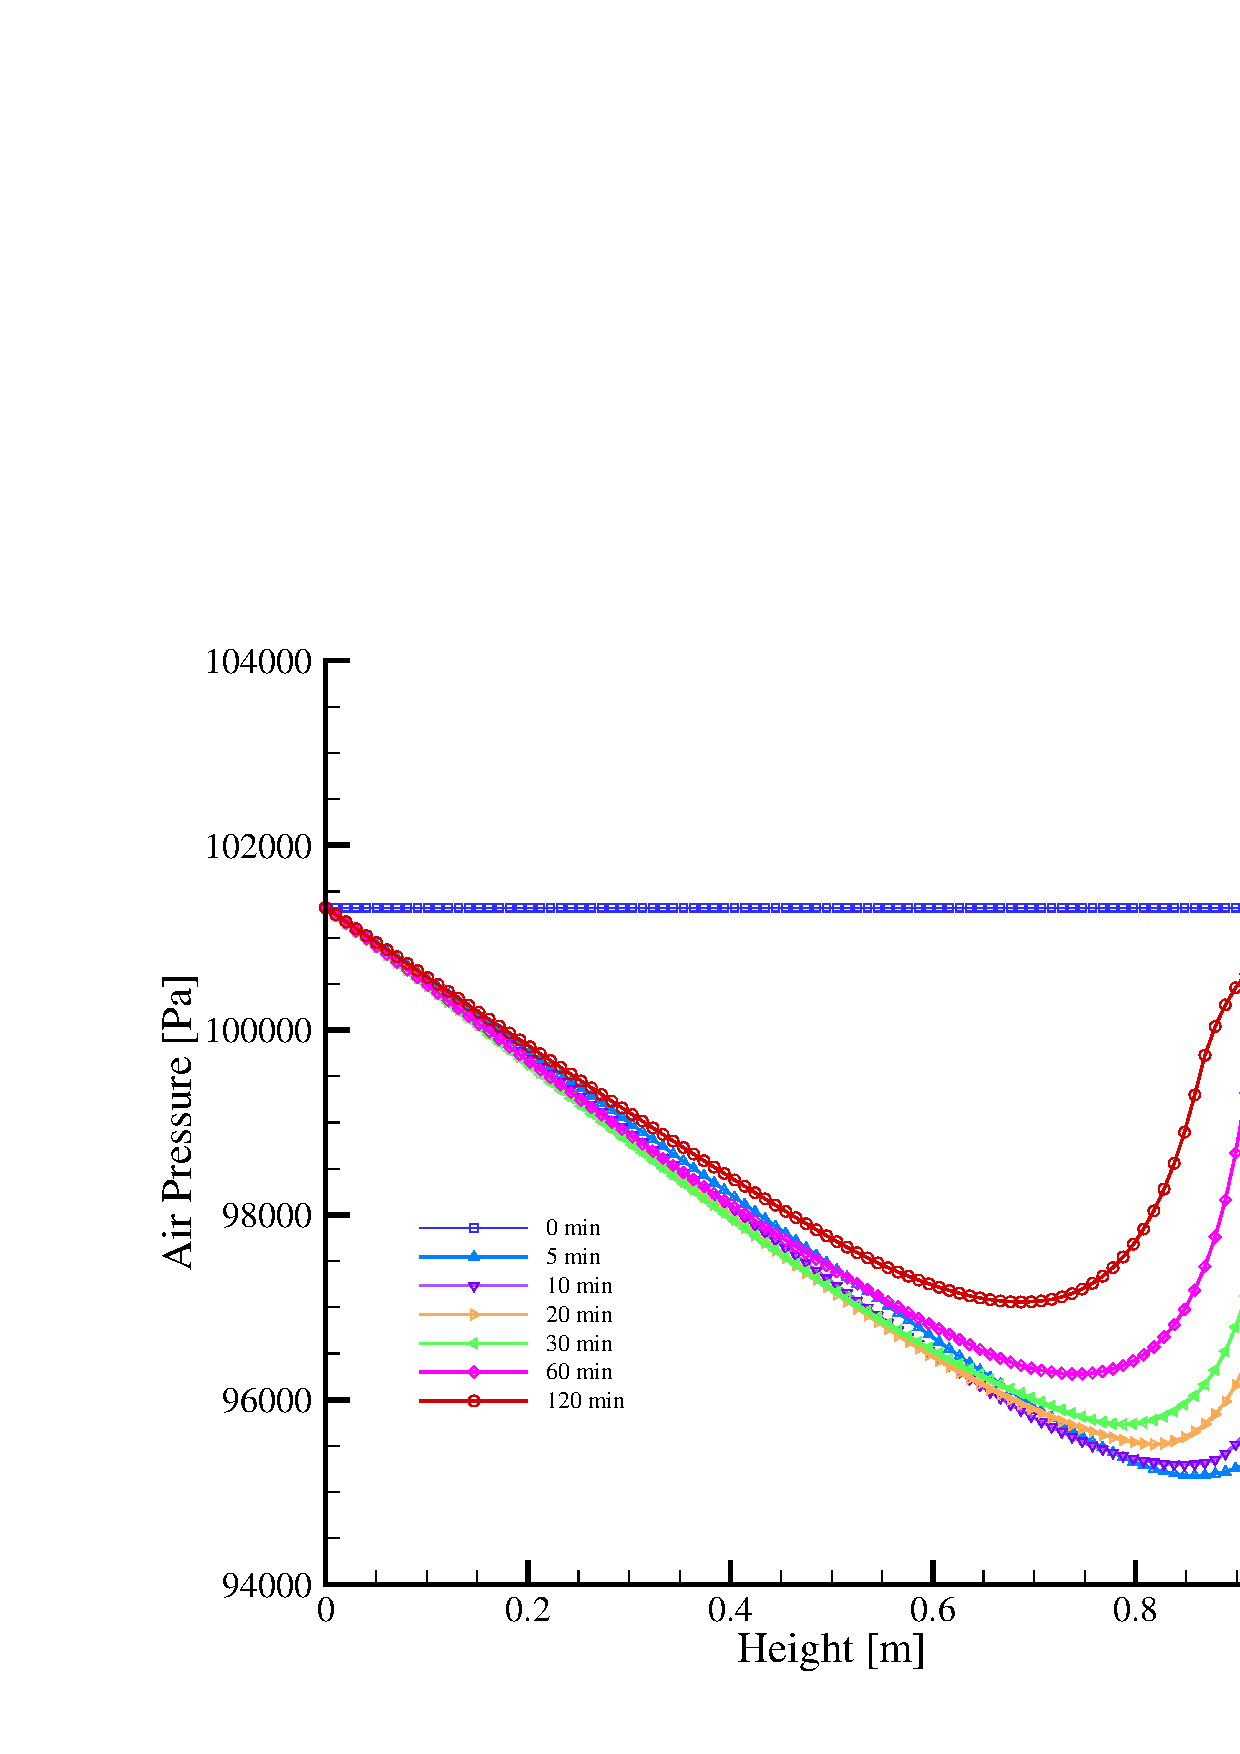
\includegraphics[scale=0.42]{chapter_13/figures/fig_13_1_2_b}
\end{center}
\caption{Vertical profiles of capillary (top) and gas pressures (bottom).}
\label{liak:p_pc}
\end{figure}

\begin{figure}[!tbh]
\begin{center}
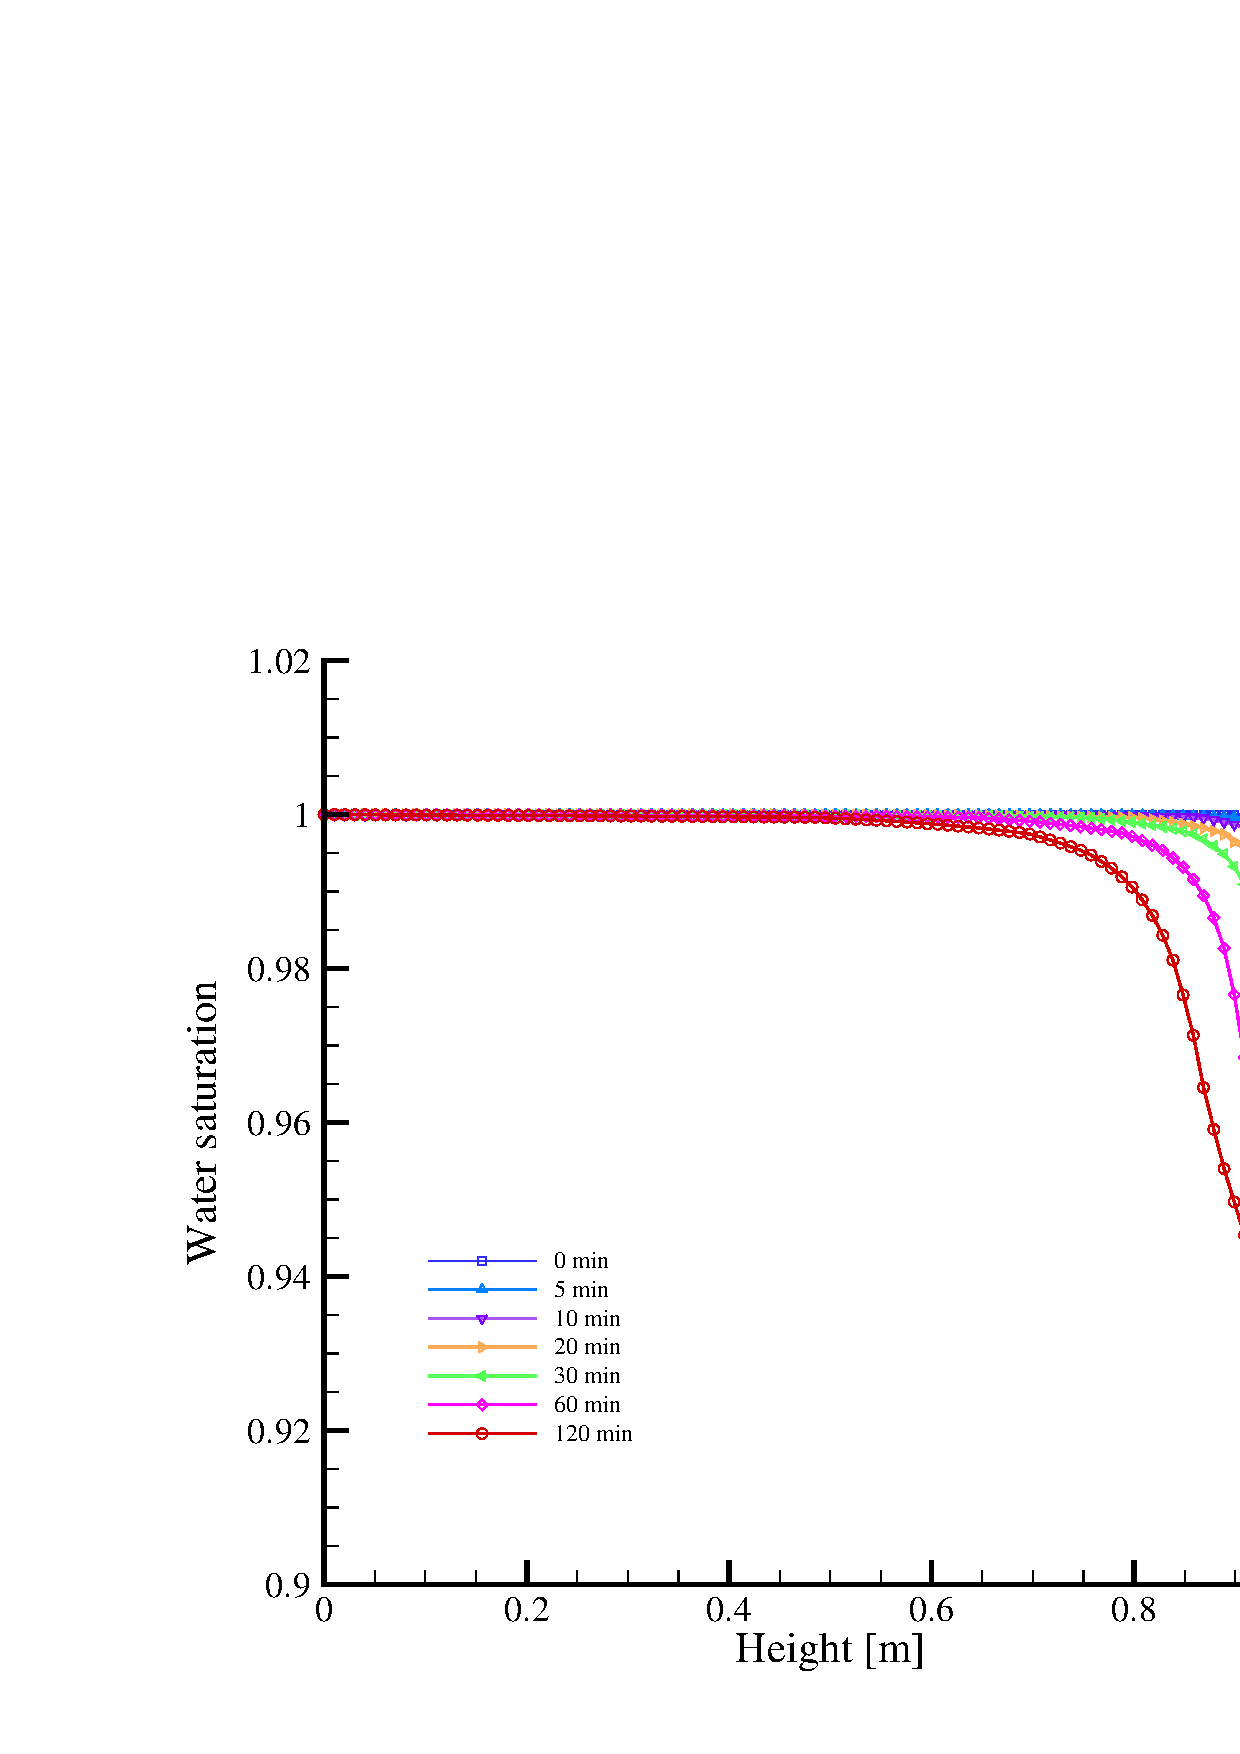
\includegraphics[scale=0.38]{chapter_13/figures/fig_13_1_3}
\end{center}
\caption{Profile of water saturation.}
\label{liak:p_sat}
\end{figure}

The results of the element test are depicted in Fig. \ref{liak:p_pce} for capillary pressure. A comparison if the results between the two-phase flow model and the Richards model can be found in Chapter 6. 

\begin{figure}[!tbh]
\begin{center}
\includegraphics[scale=0.38]{chapter_13/figures/fig_13_1_4}
\end{center}
\caption{Results of element test.}
\label{liak:p_pce}
\end{figure}

